% plan.tex — multi-backend compute framework (WGPU) migration
% Compile: pdflatex plan.tex  (twice)
% NOTE (2026-08-24): no TeX engine on this host; plan.pdf is a declared waiver
% (tools.yaml docs.latex.status = absent). This source compiles as-is.
\documentclass[11pt,a4paper]{article}

\usepackage[margin=25mm]{geometry}
\usepackage{amsmath}
\usepackage{booktabs}
\usepackage{longtable}
\usepackage{tikz}
\usepackage{listings}
\usetikzlibrary{arrows.meta,positioning,fit,backgrounds,calc}
\usepackage[hidelinks]{hyperref}

\title{Multi-Backend Compute Framework for HyMeKo\\
       \large Phase 0 audit and staged migration plan}
\author{HyMeKo semantic core workspace}
\date{Created-at: 2026-08-24 05:41 CEST}

\begin{document}
\maketitle

\section{Scope}

Evolve the existing HyMeKo tensor / HNN execution layer into a layered,
multi-backend compute framework in which the current serial/Rayon
implementation is the first CPU backend and WGPU/WGSL is the second, without
losing the measured CPU optimisations already in the working tree.

Full audit, component classification and migration classification live in
\texttt{docs/compute-framework.md}. This document is the plan-of-record
required by CLAUDE.md \S2; it does not duplicate that content.

\paragraph{Authorisation.}
\begin{quote}
\texttt{APPROVED-ARCHITECTURE-EVOLUTION: hymeko-compute-framework-wgpu}
\end{quote}

\paragraph{Estimated time of completion (ETA).}
Phase 0: complete ($\approx$1.5\,h --- audit, backup, feasibility diagnosis,
this bundle). Phase 1 skeleton: $\approx$3\,h. Phase 2 (SpMM kernel +
correctness + benchmarks): $\approx$5\,h. Phases 3--5 are gated on Phase 2
results and are not estimated yet, deliberately.

\section{Non-goals for this round}

Stated explicitly because each was considered and rejected:

\begin{itemize}
  \item no second framework parallel to the existing tensor/HNN system;
  \item no copying of existing algorithms into new modules;
  \item no repository-wide refactor;
  \item no abstraction without a concrete consumer;
  \item no dynamic dispatch in the CPU hot path;
  \item no change to the known 57/58 fixture drift.
\end{itemize}

\section{Affected files}

\subsection*{Phase 0 (this bundle) --- documentation only}
\texttt{docs/compute-framework.md}, \texttt{docs/plans/2026-08-24-compute-framework/*}.
\textbf{No source file was modified.}

\subsection*{Phase 1--2 (planned)}
\begin{itemize}
  \item \texttt{hymeko\_core/src/tensor/compute/*} --- new, dependency-free
        vocabulary (\textbf{core, needs its own token}, see \S\ref{sec:risk});
  \item \texttt{hymeko\_wgpu/*} --- new crate;
  \item \texttt{hymeko\_framework/vendor/*} --- 64 additive crate directories
        (\textbf{outside this workspace}, needs authorisation);
  \item benchmarks and tests under already-allowlisted paths.
\end{itemize}

\section{Architecture}

Target layering, with the existing code as the first backend rather than as
something to be replaced:

% plan.tikz — target layering for the multi-backend compute framework.
% % plan.tikz — target layering for the multi-backend compute framework.
% % plan.tikz — target layering for the multi-backend compute framework.
% \input{plan.tikz} from plan.tex, or wrap in a minimal standalone document
% with \usepackage{tikz} and \usetikzlibrary{arrows.meta,positioning,fit,backgrounds,calc}.

\begin{figure}[htbp]
\centering
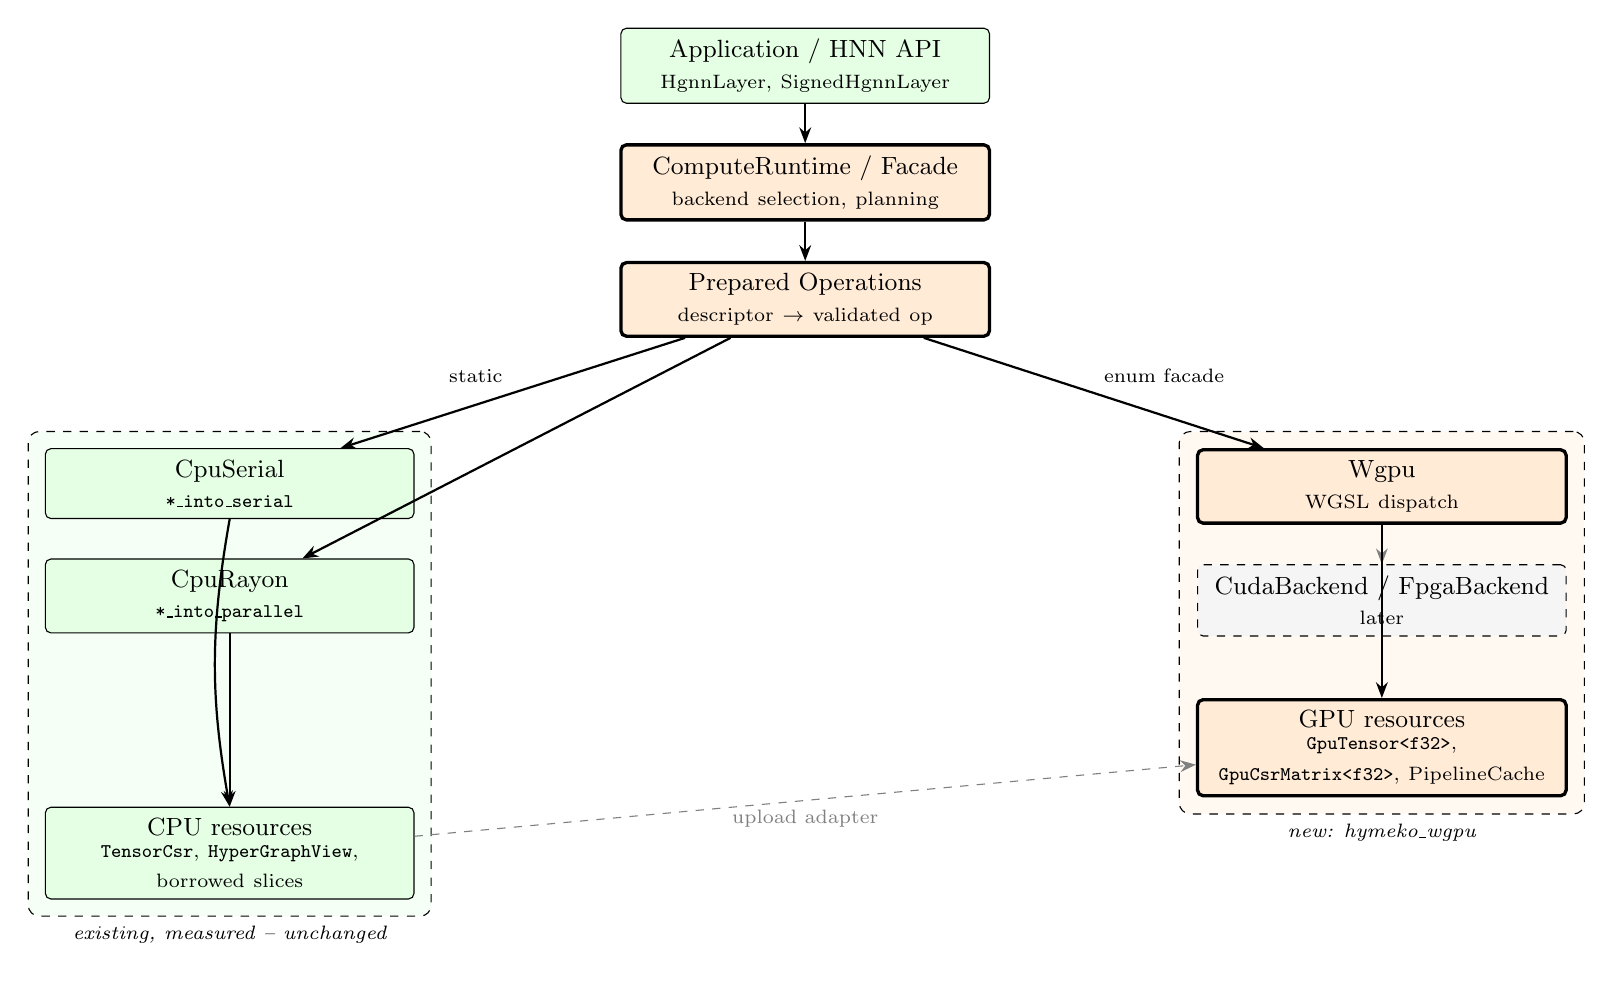
\begin{tikzpicture}[
  font=\small,
  node distance=5mm and 9mm,
  layer/.style={draw, rounded corners=2pt, align=center, inner sep=4pt,
                minimum height=8mm, text width=44mm},
  exist/.style={layer, fill=green!10},
  newc/.style={layer, fill=orange!16, very thick},
  future/.style={layer, fill=gray!8, dashed},
  flow/.style={-{Stealth[length=2mm]}, thick},
  weak/.style={-{Stealth[length=2mm]}, dashed, gray}
]

\node[exist] (app) {Application / HNN API\\{\scriptsize HgnnLayer, SignedHgnnLayer}};
\node[newc, below=of app] (facade) {ComputeRuntime / Facade\\{\scriptsize backend selection, planning}};
\node[newc, below=of facade] (prep) {Prepared Operations\\{\scriptsize descriptor $\rightarrow$ validated op}};

\draw[flow] (app) -- (facade);
\draw[flow] (facade) -- (prep);

% --- strategies -----------------------------------------------------
\node[exist, below left=14mm and 26mm of prep] (ser) {CpuSerial\\{\scriptsize \texttt{*\_into\_serial}}};
\node[exist, below=of ser] (par) {CpuRayon\\{\scriptsize \texttt{*\_into\_parallel}}};
\node[newc, below right=14mm and 26mm of prep] (wgpu) {Wgpu\\{\scriptsize WGSL dispatch}};
\node[future, below=of wgpu] (cuda) {CudaBackend / FpgaBackend\\{\scriptsize later}};

\draw[flow] (prep) -- node[above left,font=\scriptsize]{static} (ser);
\draw[flow] (prep) -- (par);
\draw[flow] (prep) -- node[above right,font=\scriptsize]{enum facade} (wgpu);
\draw[weak] (wgpu) -- (cuda);

% --- resources ------------------------------------------------------
\node[exist, below=22mm of par] (cpures) {CPU resources\\{\scriptsize \texttt{TensorCsr}, \texttt{HyperGraphView},\\ borrowed slices}};
\node[newc, below=22mm of wgpu] (gpures) {GPU resources\\{\scriptsize \texttt{GpuTensor<f32>},\\\texttt{GpuCsrMatrix<f32>}, PipelineCache}};

\draw[flow] (ser.south) to[bend right=10] (cpures.north);
\draw[flow] (par) -- (cpures);
\draw[flow] (wgpu) -- (gpures);
\draw[weak] (cpures) -- node[below,font=\scriptsize]{upload adapter} (gpures);

\begin{scope}[on background layer]
  \node[draw, dashed, fill=green!4, inner sep=6pt, rounded corners,
        fit=(ser)(par)(cpures),
        label={[font=\scriptsize\itshape]below:existing, measured -- unchanged}] {};
  \node[draw, dashed, fill=orange!5, inner sep=6pt, rounded corners,
        fit=(wgpu)(gpures),
        label={[font=\scriptsize\itshape]below:new: hymeko\_wgpu}] {};
\end{scope}

\end{tikzpicture}
\caption{Target layering. The green region is the \emph{existing} CPU
implementation, which becomes the first backend rather than being rewritten:
\texttt{CpuSerial} and \texttt{CpuRayon} are the already-measured
\texttt{*\_into\_serial} / \texttt{*\_into\_parallel} kernels, reached through
static dispatch so the hot path keeps its current codegen. Only the outermost
device choice uses an enum, paid once per invocation. Core tensor types never
acquire a device handle; an upload \emph{adapter} produces the GPU
representation instead.}
\end{figure}

\begin{figure}[htbp]
\centering
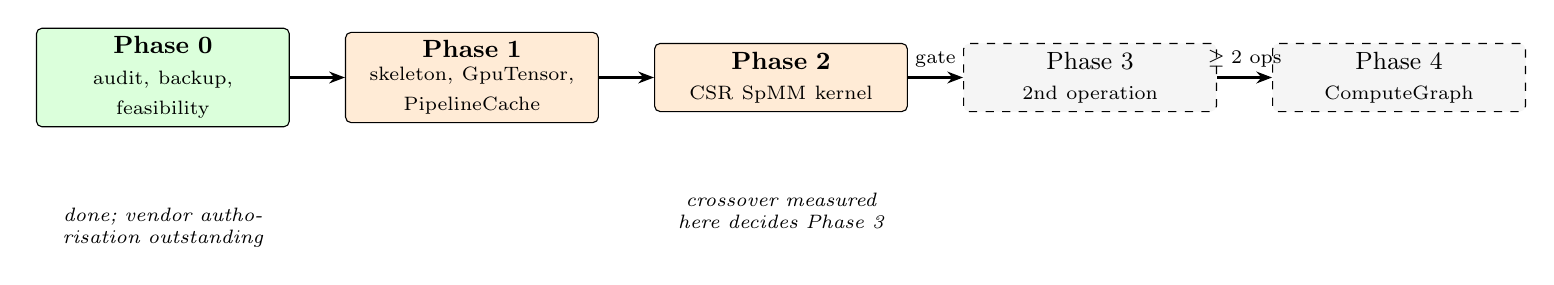
\begin{tikzpicture}[
  font=\small,
  ph/.style={draw, rounded corners=2pt, align=center, inner sep=3pt,
             minimum height=7mm, text width=30mm},
  done/.style={ph, fill=green!14},
  ready/.style={ph, fill=orange!16},
  gated/.style={ph, fill=gray!8, dashed},
  flow/.style={-{Stealth[length=2mm]}, thick},
  node distance=7mm
]

\node[done] (p0) {\textbf{Phase 0}\\{\scriptsize audit, backup, feasibility}};
\node[ready, right=of p0] (p1) {\textbf{Phase 1}\\{\scriptsize skeleton, GpuTensor,\\PipelineCache}};
\node[ready, right=of p1] (p2) {\textbf{Phase 2}\\{\scriptsize CSR SpMM kernel}};
\node[gated, right=of p2] (p3) {Phase 3\\{\scriptsize 2nd operation}};
\node[gated, right=of p3] (p4) {Phase 4\\{\scriptsize ComputeGraph}};

\draw[flow] (p0) -- (p1);
\draw[flow] (p1) -- (p2);
\draw[flow] (p2) -- node[above,font=\scriptsize]{gate} (p3);
\draw[flow] (p3) -- node[above,font=\scriptsize]{$\ge 2$ ops} (p4);

\node[below=9mm of p0, font=\scriptsize\itshape, text width=32mm, align=center]
  {done; vendor authorisation outstanding};
\node[below=9mm of p2, font=\scriptsize\itshape, text width=34mm, align=center]
  {crossover measured here decides Phase 3};

\end{tikzpicture}
\caption{Phase gating. Phases 3 and 4 are deliberately not scheduled: the
second operation is chosen from \emph{measured} Phase 2 results, and the compute
graph is not introduced until at least two GPU operations exist to compose ---
avoiding an abstraction with no consumer.}
\end{figure}
 from plan.tex, or wrap in a minimal standalone document
% with \usepackage{tikz} and \usetikzlibrary{arrows.meta,positioning,fit,backgrounds,calc}.

\begin{figure}[htbp]
\centering
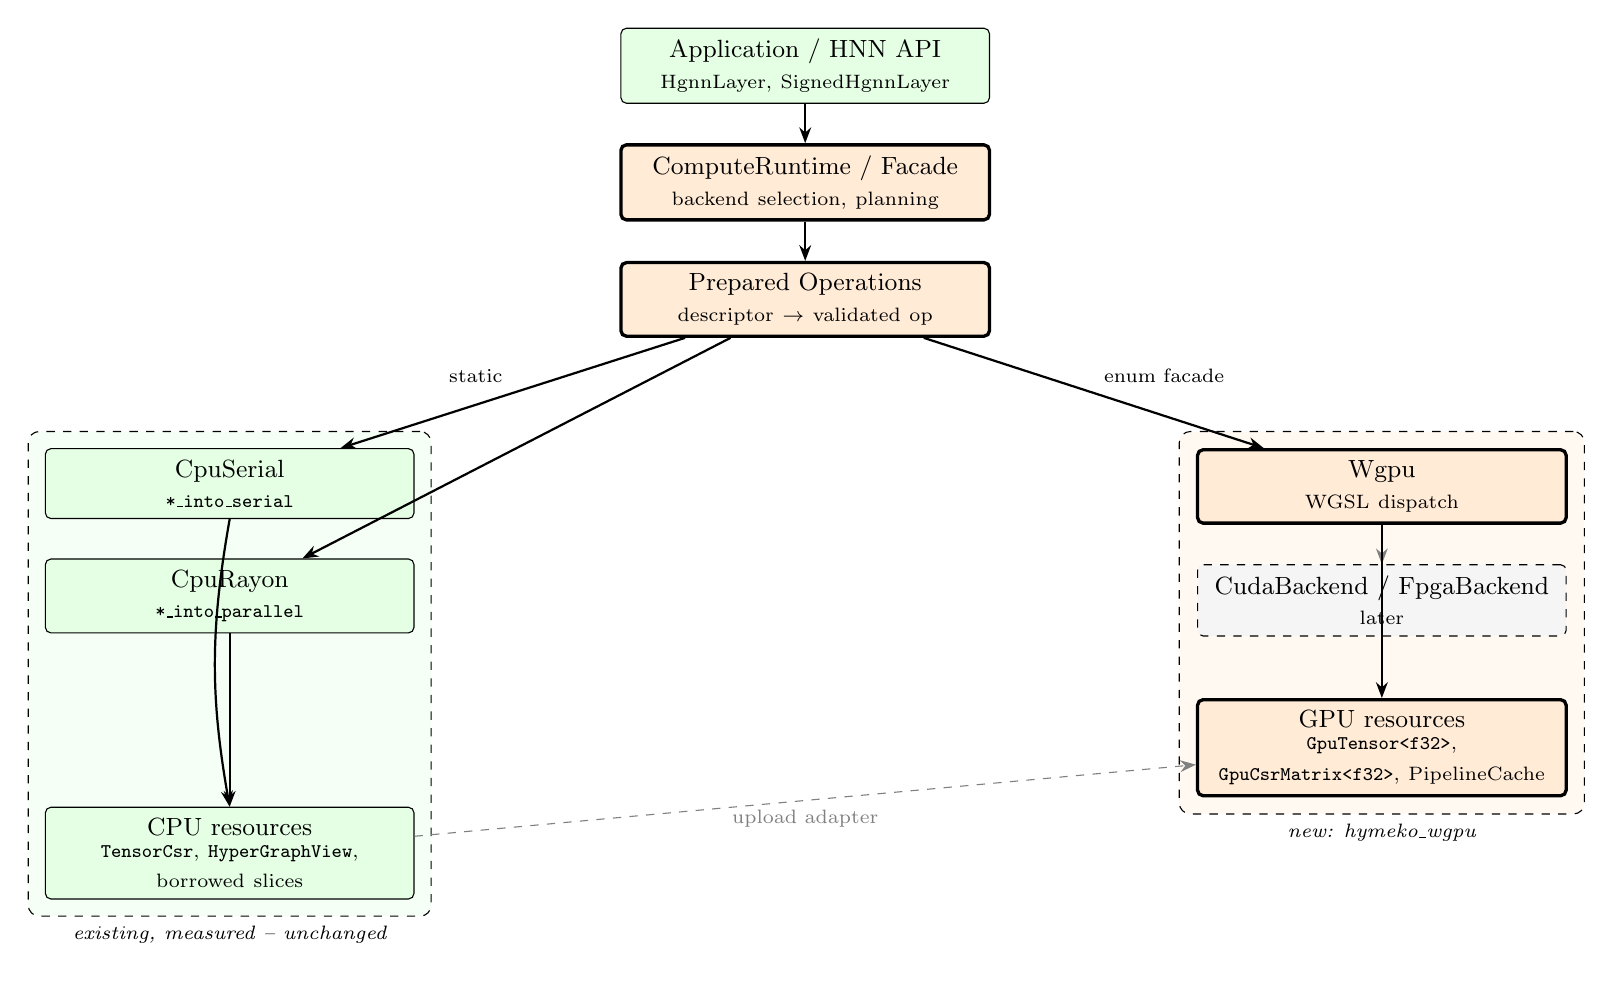
\begin{tikzpicture}[
  font=\small,
  node distance=5mm and 9mm,
  layer/.style={draw, rounded corners=2pt, align=center, inner sep=4pt,
                minimum height=8mm, text width=44mm},
  exist/.style={layer, fill=green!10},
  newc/.style={layer, fill=orange!16, very thick},
  future/.style={layer, fill=gray!8, dashed},
  flow/.style={-{Stealth[length=2mm]}, thick},
  weak/.style={-{Stealth[length=2mm]}, dashed, gray}
]

\node[exist] (app) {Application / HNN API\\{\scriptsize HgnnLayer, SignedHgnnLayer}};
\node[newc, below=of app] (facade) {ComputeRuntime / Facade\\{\scriptsize backend selection, planning}};
\node[newc, below=of facade] (prep) {Prepared Operations\\{\scriptsize descriptor $\rightarrow$ validated op}};

\draw[flow] (app) -- (facade);
\draw[flow] (facade) -- (prep);

% --- strategies -----------------------------------------------------
\node[exist, below left=14mm and 26mm of prep] (ser) {CpuSerial\\{\scriptsize \texttt{*\_into\_serial}}};
\node[exist, below=of ser] (par) {CpuRayon\\{\scriptsize \texttt{*\_into\_parallel}}};
\node[newc, below right=14mm and 26mm of prep] (wgpu) {Wgpu\\{\scriptsize WGSL dispatch}};
\node[future, below=of wgpu] (cuda) {CudaBackend / FpgaBackend\\{\scriptsize later}};

\draw[flow] (prep) -- node[above left,font=\scriptsize]{static} (ser);
\draw[flow] (prep) -- (par);
\draw[flow] (prep) -- node[above right,font=\scriptsize]{enum facade} (wgpu);
\draw[weak] (wgpu) -- (cuda);

% --- resources ------------------------------------------------------
\node[exist, below=22mm of par] (cpures) {CPU resources\\{\scriptsize \texttt{TensorCsr}, \texttt{HyperGraphView},\\ borrowed slices}};
\node[newc, below=22mm of wgpu] (gpures) {GPU resources\\{\scriptsize \texttt{GpuTensor<f32>},\\\texttt{GpuCsrMatrix<f32>}, PipelineCache}};

\draw[flow] (ser.south) to[bend right=10] (cpures.north);
\draw[flow] (par) -- (cpures);
\draw[flow] (wgpu) -- (gpures);
\draw[weak] (cpures) -- node[below,font=\scriptsize]{upload adapter} (gpures);

\begin{scope}[on background layer]
  \node[draw, dashed, fill=green!4, inner sep=6pt, rounded corners,
        fit=(ser)(par)(cpures),
        label={[font=\scriptsize\itshape]below:existing, measured -- unchanged}] {};
  \node[draw, dashed, fill=orange!5, inner sep=6pt, rounded corners,
        fit=(wgpu)(gpures),
        label={[font=\scriptsize\itshape]below:new: hymeko\_wgpu}] {};
\end{scope}

\end{tikzpicture}
\caption{Target layering. The green region is the \emph{existing} CPU
implementation, which becomes the first backend rather than being rewritten:
\texttt{CpuSerial} and \texttt{CpuRayon} are the already-measured
\texttt{*\_into\_serial} / \texttt{*\_into\_parallel} kernels, reached through
static dispatch so the hot path keeps its current codegen. Only the outermost
device choice uses an enum, paid once per invocation. Core tensor types never
acquire a device handle; an upload \emph{adapter} produces the GPU
representation instead.}
\end{figure}

\begin{figure}[htbp]
\centering
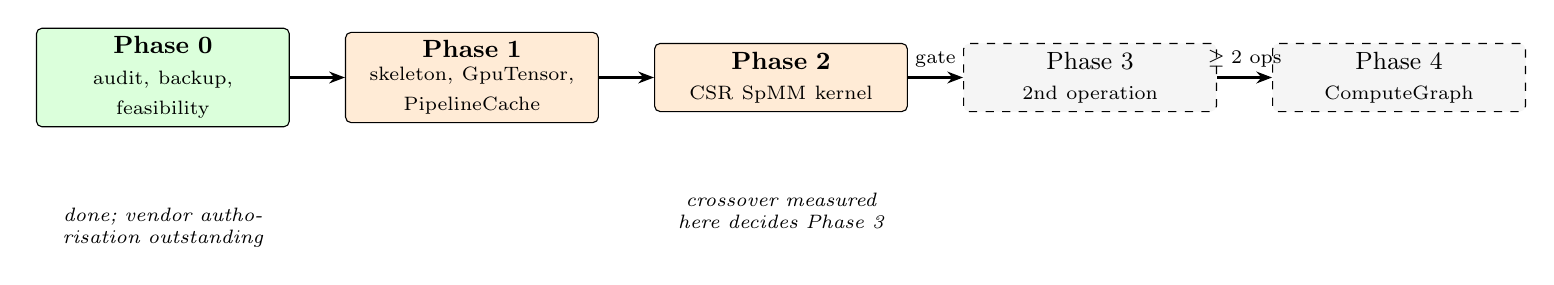
\begin{tikzpicture}[
  font=\small,
  ph/.style={draw, rounded corners=2pt, align=center, inner sep=3pt,
             minimum height=7mm, text width=30mm},
  done/.style={ph, fill=green!14},
  ready/.style={ph, fill=orange!16},
  gated/.style={ph, fill=gray!8, dashed},
  flow/.style={-{Stealth[length=2mm]}, thick},
  node distance=7mm
]

\node[done] (p0) {\textbf{Phase 0}\\{\scriptsize audit, backup, feasibility}};
\node[ready, right=of p0] (p1) {\textbf{Phase 1}\\{\scriptsize skeleton, GpuTensor,\\PipelineCache}};
\node[ready, right=of p1] (p2) {\textbf{Phase 2}\\{\scriptsize CSR SpMM kernel}};
\node[gated, right=of p2] (p3) {Phase 3\\{\scriptsize 2nd operation}};
\node[gated, right=of p3] (p4) {Phase 4\\{\scriptsize ComputeGraph}};

\draw[flow] (p0) -- (p1);
\draw[flow] (p1) -- (p2);
\draw[flow] (p2) -- node[above,font=\scriptsize]{gate} (p3);
\draw[flow] (p3) -- node[above,font=\scriptsize]{$\ge 2$ ops} (p4);

\node[below=9mm of p0, font=\scriptsize\itshape, text width=32mm, align=center]
  {done; vendor authorisation outstanding};
\node[below=9mm of p2, font=\scriptsize\itshape, text width=34mm, align=center]
  {crossover measured here decides Phase 3};

\end{tikzpicture}
\caption{Phase gating. Phases 3 and 4 are deliberately not scheduled: the
second operation is chosen from \emph{measured} Phase 2 results, and the compute
graph is not introduced until at least two GPU operations exist to compose ---
avoiding an abstraction with no consumer.}
\end{figure}
 from plan.tex, or wrap in a minimal standalone document
% with \usepackage{tikz} and \usetikzlibrary{arrows.meta,positioning,fit,backgrounds,calc}.

\begin{figure}[htbp]
\centering
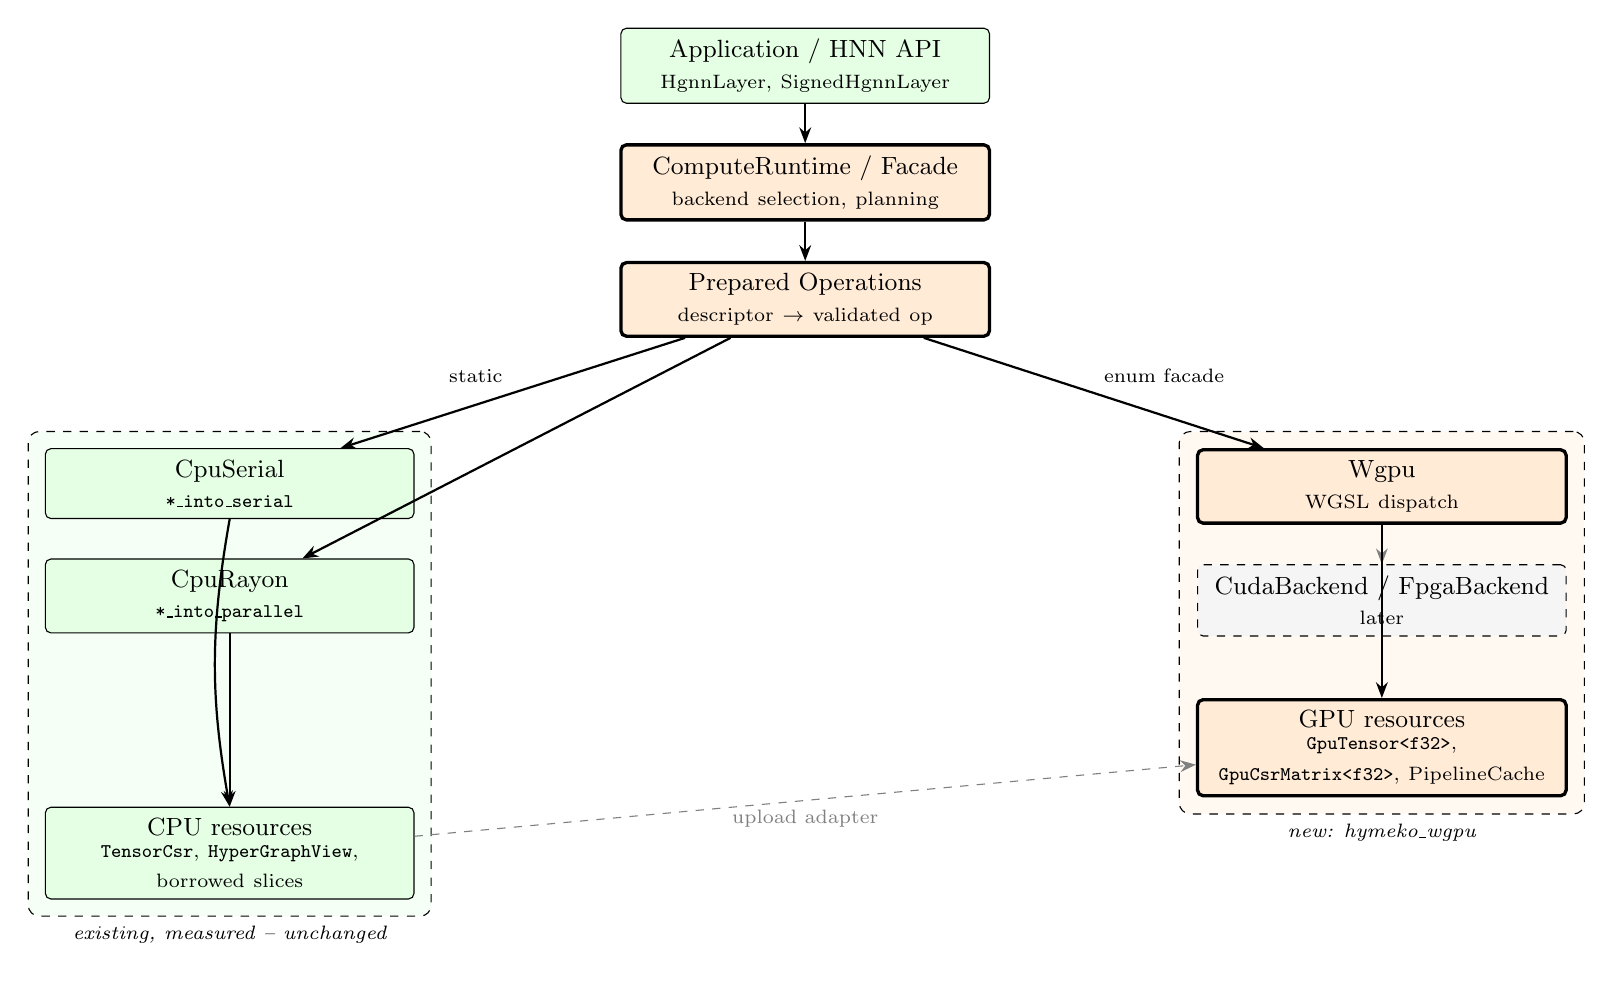
\begin{tikzpicture}[
  font=\small,
  node distance=5mm and 9mm,
  layer/.style={draw, rounded corners=2pt, align=center, inner sep=4pt,
                minimum height=8mm, text width=44mm},
  exist/.style={layer, fill=green!10},
  newc/.style={layer, fill=orange!16, very thick},
  future/.style={layer, fill=gray!8, dashed},
  flow/.style={-{Stealth[length=2mm]}, thick},
  weak/.style={-{Stealth[length=2mm]}, dashed, gray}
]

\node[exist] (app) {Application / HNN API\\{\scriptsize HgnnLayer, SignedHgnnLayer}};
\node[newc, below=of app] (facade) {ComputeRuntime / Facade\\{\scriptsize backend selection, planning}};
\node[newc, below=of facade] (prep) {Prepared Operations\\{\scriptsize descriptor $\rightarrow$ validated op}};

\draw[flow] (app) -- (facade);
\draw[flow] (facade) -- (prep);

% --- strategies -----------------------------------------------------
\node[exist, below left=14mm and 26mm of prep] (ser) {CpuSerial\\{\scriptsize \texttt{*\_into\_serial}}};
\node[exist, below=of ser] (par) {CpuRayon\\{\scriptsize \texttt{*\_into\_parallel}}};
\node[newc, below right=14mm and 26mm of prep] (wgpu) {Wgpu\\{\scriptsize WGSL dispatch}};
\node[future, below=of wgpu] (cuda) {CudaBackend / FpgaBackend\\{\scriptsize later}};

\draw[flow] (prep) -- node[above left,font=\scriptsize]{static} (ser);
\draw[flow] (prep) -- (par);
\draw[flow] (prep) -- node[above right,font=\scriptsize]{enum facade} (wgpu);
\draw[weak] (wgpu) -- (cuda);

% --- resources ------------------------------------------------------
\node[exist, below=22mm of par] (cpures) {CPU resources\\{\scriptsize \texttt{TensorCsr}, \texttt{HyperGraphView},\\ borrowed slices}};
\node[newc, below=22mm of wgpu] (gpures) {GPU resources\\{\scriptsize \texttt{GpuTensor<f32>},\\\texttt{GpuCsrMatrix<f32>}, PipelineCache}};

\draw[flow] (ser.south) to[bend right=10] (cpures.north);
\draw[flow] (par) -- (cpures);
\draw[flow] (wgpu) -- (gpures);
\draw[weak] (cpures) -- node[below,font=\scriptsize]{upload adapter} (gpures);

\begin{scope}[on background layer]
  \node[draw, dashed, fill=green!4, inner sep=6pt, rounded corners,
        fit=(ser)(par)(cpures),
        label={[font=\scriptsize\itshape]below:existing, measured -- unchanged}] {};
  \node[draw, dashed, fill=orange!5, inner sep=6pt, rounded corners,
        fit=(wgpu)(gpures),
        label={[font=\scriptsize\itshape]below:new: hymeko\_wgpu}] {};
\end{scope}

\end{tikzpicture}
\caption{Target layering. The green region is the \emph{existing} CPU
implementation, which becomes the first backend rather than being rewritten:
\texttt{CpuSerial} and \texttt{CpuRayon} are the already-measured
\texttt{*\_into\_serial} / \texttt{*\_into\_parallel} kernels, reached through
static dispatch so the hot path keeps its current codegen. Only the outermost
device choice uses an enum, paid once per invocation. Core tensor types never
acquire a device handle; an upload \emph{adapter} produces the GPU
representation instead.}
\end{figure}

\begin{figure}[htbp]
\centering
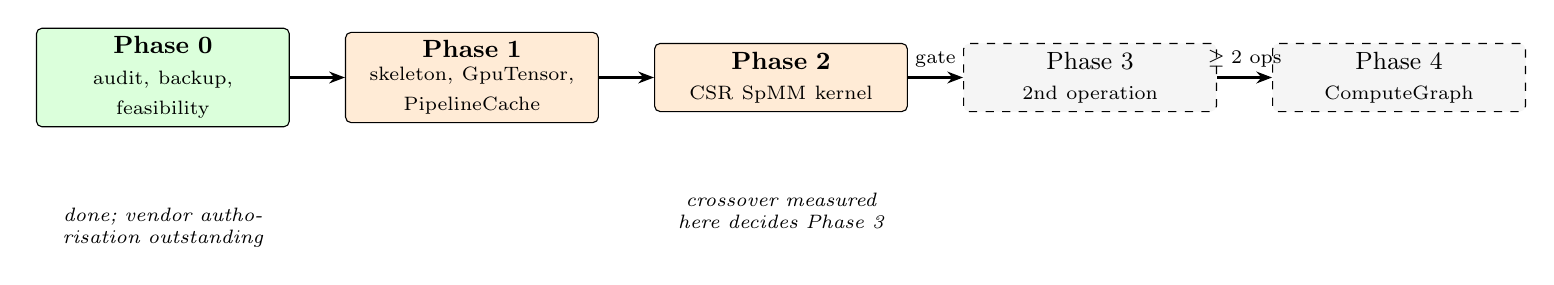
\begin{tikzpicture}[
  font=\small,
  ph/.style={draw, rounded corners=2pt, align=center, inner sep=3pt,
             minimum height=7mm, text width=30mm},
  done/.style={ph, fill=green!14},
  ready/.style={ph, fill=orange!16},
  gated/.style={ph, fill=gray!8, dashed},
  flow/.style={-{Stealth[length=2mm]}, thick},
  node distance=7mm
]

\node[done] (p0) {\textbf{Phase 0}\\{\scriptsize audit, backup, feasibility}};
\node[ready, right=of p0] (p1) {\textbf{Phase 1}\\{\scriptsize skeleton, GpuTensor,\\PipelineCache}};
\node[ready, right=of p1] (p2) {\textbf{Phase 2}\\{\scriptsize CSR SpMM kernel}};
\node[gated, right=of p2] (p3) {Phase 3\\{\scriptsize 2nd operation}};
\node[gated, right=of p3] (p4) {Phase 4\\{\scriptsize ComputeGraph}};

\draw[flow] (p0) -- (p1);
\draw[flow] (p1) -- (p2);
\draw[flow] (p2) -- node[above,font=\scriptsize]{gate} (p3);
\draw[flow] (p3) -- node[above,font=\scriptsize]{$\ge 2$ ops} (p4);

\node[below=9mm of p0, font=\scriptsize\itshape, text width=32mm, align=center]
  {done; vendor authorisation outstanding};
\node[below=9mm of p2, font=\scriptsize\itshape, text width=34mm, align=center]
  {crossover measured here decides Phase 3};

\end{tikzpicture}
\caption{Phase gating. Phases 3 and 4 are deliberately not scheduled: the
second operation is chosen from \emph{measured} Phase 2 results, and the compute
graph is not introduced until at least two GPU operations exist to compose ---
avoiding an abstraction with no consumer.}
\end{figure}


\section{Design patterns --- selected and rejected}

\begin{longtable}{p{0.24\textwidth}p{0.34\textwidth}p{0.34\textwidth}}
\toprule
\textbf{Pattern} & \textbf{Where} & \textbf{Justification} \\
\midrule
Abstract Factory & backend creates its own resources
& A GPU tensor cannot be constructed without a device; the backend is the only
  thing that knows the device. No general factory hierarchy. \\
\addlinespace
Builder & \texttt{WgpuBackend::builder()}, \texttt{SpmmBuilder}
& Device acquisition is fallible and async; operation preparation needs
  validation before any GPU resource is committed. \\
\addlinespace
Command & \texttt{operation.encode(\&mut encoder)}
& Multiple operations must share one command buffer and one submit. Automatic
  submit-per-operation is the single biggest GPU anti-pattern to avoid. \\
\addlinespace
Strategy (static) & CPU serial / CPU Rayon
& Already implemented as \texttt{*\_into\_serial} / \texttt{*\_into\_parallel};
  monomorphised, zero hot-loop cost. \\
\addlinespace
Adapter & \texttt{TensorCsr} $\rightarrow$ \texttt{GpuCsrMatrix}
& Keeps device handles out of core types, which the task requires. \\
\addlinespace
Flyweight & \texttt{PipelineCache}
& Pipeline creation is orders of magnitude more expensive than dispatch; it
  must not recur per call. \\
\addlinespace
Facade & \texttt{runtime.spmm(...)}
& Convenience over, not instead of, the explicit
  upload/prepare/encode/submit/readback path. \\
\midrule
\textbf{Rejected} & & \\
\midrule
\texttt{Box<dyn Backend>} & --- & Erases \texttt{F: Real}, forfeits mixed
  precision, and blocks monomorphisation. Rejected in
  \texttt{docs/backend-abstraction.md} \S2 and still rejected. \\
\addlinespace
Universal erased \texttt{Tensor} & --- & Round 1 keeps the f32 GPU path
  explicit; a type-erasing container would hide exactly the information the
  first kernel needs. \\
\addlinespace
\texttt{ComputeGraph} (now) & --- & Deferred until $\ge$2 working GPU
  operations exist, per the task's own gate. \\
\addlinespace
Separate \texttt{hymeko\_compute} crate & --- & Deferred until $\ge$3 backends;
  see \texttt{docs/compute-framework.md} \S4 for the dependency-edge argument. \\
\bottomrule
\end{longtable}

\section{Test strategy}

\begin{description}
  \item[Unchanged] the 31 CPU regression tests keep their \emph{bitwise}
    assertions. The framework layer may not weaken one of them.
  \item[New, CPU] one benchmark cell calling SpMM through the structured
    operation, compared against the direct \texttt{spmm\_into} call. Acceptance:
    within noise. A measurable gap fails the abstraction.
  \item[New, GPU] empty; singleton; empty row; irregular degree; duplicate
    column; negative and zero values; \texttt{feature\_dim} $\in
    \{1,8,32,128\}$; shapes not divisible by the workgroup size; mismatched
    input/output shapes; repeated dispatch of one prepared operation; dispatch
    after input update.
  \item[CPU vs GPU] absolute \emph{and} relative tolerance, explicit NaN/Inf
    handling. \textbf{Bitwise equality is not promised across devices} ---
    segmented reductions reassociate.
  \item[Adapter absence] a missing adapter is a documented skip; a shader
    compilation failure or a numerical mismatch is \textbf{never} a skip.
\end{description}

\section{Performance budget}

\begin{itemize}
  \item Structured CPU operation: within measurement noise of \texttt{spmm\_into}.
  \item No previously measured cell may regress by $>$10\,\% (\S3 gate).
  \item Pipeline built once per configuration, never per dispatch.
  \item Bind groups rebuilt only when buffers change.
  \item Static CSR uploaded once and reused across dispatches.
  \item Readback only at an explicit boundary; no busy-poll on device.
\end{itemize}

\section{Risk anticipation}
\label{sec:risk}

\begin{description}
  \item[Inherited environment claims.] Phase 0's headline risk already
    materialised: a checked-in comment asserting crates.io was unreachable was
    \emph{false}, and four commands falsified it. Trusting it would have cost a
    hand-vendoring campaign. Treat environment assertions in config files as
    timestamped hypotheses.
  \item[Shared vendor tree.] \texttt{hymeko\_framework/vendor/} is used by five
    sibling repositories. Only an \emph{additive} copy of the 64 missing crates
    is proposed; regenerating the tree could drop crates only the siblings need.
  \item[Core lockdown.] Putting the backend vocabulary in
    \texttt{hymeko\_core::tensor::compute} touches a \texttt{lockdown: full}
    crate and needs its own \texttt{APPROVED-CORE-EDIT}. The fallback (put it in
    \texttt{hymeko\_hnn}) avoids that but drags the hypergraph layer into the GPU
    crate's dependency set. Escalate rather than choose silently.
  \item[Abstraction overhead.] The stated failure mode is a framework layer that
    is measurably slower than the direct call. Mitigated by the dedicated
    benchmark cell above, run \emph{before} the abstraction is accepted.
  \item[Measurement drift.] The CPU round documented a $\approx$20\,\%
    run-to-run band on small cells under sustained load on this laptop. GPU
    benchmarking heats it further; small-cell CPU/GPU comparisons must be run
    back-to-back and inconclusive results reported as such.
  \item[Worst-case input.] Large workload: $\approx$200k nodes / 100k edges /
    1.2M incidences, CSR $\approx$4M nnz, \texttt{feature\_dim} up to 128 ---
    $\approx$256\,MB of f32 per dense side at the largest cell, which must fit
    device memory alongside the CSR.
\end{description}

\section{Rollback path}

Phase 0 modified no source. Phases 1--2 are additive: a new crate and a new
module. Rollback is deleting \texttt{hymeko\_wgpu/}, reverting the manifest
entry, and (if desired) removing the 64 vendored directories. The CPU path is
untouched throughout by construction --- the GPU backend is a new consumer of
existing kernels, never a replacement for them.

\end{document}
